\باب{حرارت نا گزر تخمین}\شناخت{باب_حرارت_نا_گزر_تخمین}

\حصہ{مسئلہ حرارت ناگزر}
\جزوحصہ{حرارت ناگزر عمل}
فرض کریں ایک کامل   رقاص   انتصابی ستہ میں بغیر کسی رگڑ یا ہوائی مزاحمت کے آگے پیچھے ارتعاش کرتا ہے اگر آپ اس   رقاص   کو جٹکے سے ہلائیں تو یہ افراتفری کے ساتھ دائروی صورت میں حرکت کرنے لگے گا لیکن اگر آپ بغیر جھٹکے کے   رقاص   کو آہستہ آہستہ ایک مقام سے دوسری مقام منتقل کریں (شکل \حوالہ{شکل_حرارت_نا_گزر_آہستہ_منتقلی})    تب   رقاص   اسی سطح یا اس کے متوازی سطح میں شائستگی اور روانی سے اسی حیطہ کے ساتھ جلھولتا رہے گا بیرونی حالات کی بہت آہستہ آہستہ تبدیلی ہی حرارت نہ گزر عمل کی پہچان ہے دھیان رہے کہ یہاں دو مختلف امتیازی وقتتوں کی بات کی جا رہی ہے نظام کی حرکت جو یہاں   رقاص   کی ارتعاش کا دوری عرصہ ہوگا کو ظاہر کرنے والا اندرونی وقت \عددی{T_i} اور نظام میں نمایاں تبدیلی مثلا لرزتے ہوئے چبوترا پر نصب   رقاص   کی صورت میں چبوترے کی لرزش کا دوری عرصہ کو ظاہر کرنے والا بیرونی وقت \عددی{T_e} حرارت ناگزر عمل میں \عددی{T_e \gg T_i} ہوگا۔

\begin{figure}
\centering
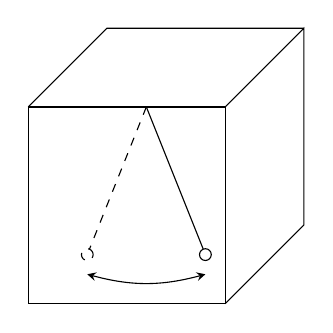
\begin{tikzpicture}[x={(-0.5cm,-0.5cm)},y={(1cm,0cm)},z={(0cm,1cm)}]
\pgfmathsetmacro{\kx}{2}
\pgfmathsetmacro{\ky}{2.5}
\pgfmathsetmacro{\kz}{2.5}
\draw[] (0,0,0) --++ (0,\ky,0) --++ (0,0,\kz) --++ (0,-\ky,0) --++ (0,0,-\kz);
\draw[] (0,\ky,0) --++ (-\kx,0,0) --++ (0,0,\kz) --++ (\kx,0,0);
\draw[] (0,0,\kz) --++ (-\kx,0,0) --++ (0,\ky,0);
\draw[] (0,0.6*\ky,\kz) --++ (0,0.3*\ky,-0.75*\kz) coordinate(a) node[circle,draw=black,fill=white, inner sep=1.5pt]{};
\draw[dashed] (0,0.6*\ky,\kz) --++ (0,-0.3*\ky,-0.75*\kz) coordinate(b) node[circle,draw=black,fill=white, inner sep=1.5pt]{};
\draw[stealth-stealth] (0,0.3*\ky,0.15*\kz) to [out=-15,in=-165] (0,0.9*\ky,0.15*\kz);
\end{tikzpicture}
\caption{حرارت نا گزر حرکت: اگر ڈبے کو نہایت آہستہ ایک جگہ سے دوسری جگہ منتقل کیا جائے تب   رقاص   اسی حیطہ کے ساتھ ابتدائی سطح کے متوازی سطح میں جھولتا ہے۔}
\label{شکل_حرارت_نا_گزر_آہستہ_منتقلی}
\end{figure}


 حرارت نہ گزر عمل کے تجزیہ کا بنیادی حکمت عملی یہ ہوگا کہ پہلے بیرونی عوامل مقدار معلوم کو غیر متغیر رکھتے ہوئے مسئلہ حل کیا جاتا ہے اور حساب کے بالکل آخر میں انہیں بہت آہستہ آہستہ وقت کے ساتھ تبدیل ہونے کی اجازت دی جاتی ہے مثال کے طور پر مقررہ لمبائی \عددی{L} کی  رقاص  کا کلاسیکی دوری عرصہ \عددی{
2 \pi \sqrt{L/g}
} ہوگا اب اگر لمبائی آہستہ آہستہ تبدیل ہو تب دوری عرصہ  بظاہر  \عددی{
2 \pi \sqrt{L(t)/g}
} ہوگا حصہ 7.3 میں ہائیڈروجن سالمہ پر تبصرہ کے دوران ایک زیادہ باریک بیں مثال پیش کی گئی ہم نے آغاز میں مرکزہ کو ساکن تصور کرتے ہوئے ان کے بیچ فاصلہ \عددی{ R} کی صورت میں الیکٹرون کی حرکت کے لئے حل کیا نظام کی زمینی حال توانائی کو \عددی{ R} کے تفاعل کی صورت میں دریافت کرنے کے بعد ہم نے توازنی فاصلہ معلوم کرکے ترسیم کی ان حنا سے مرکزہ کی لرزش کا تعدد حاصل کیا سوال 7.10 طبیعت سالمہ میں اس ترکیب کو جس میں ساکن مرکزہ سے آغاز کرتے ہوئے الیکٹرانی تفاعلات موج کا حساب کر کے ان سے نسبتا سست رفتار مرکزہ کی مقامات اور حرکت کے بارے میں معلومات حاصل کرنے کو بارن و اوپن ہائيمر تخمین کہتے ہیں حرارت نہ گزر تخمین کے بنیادی تصور کو ایک مسئلہ کے روپ میں پیش کیا جا سکتا ہے فرض کریں ہيملٹنی ابتدائی روپ \عددی{H^i} سے بہت آہستہ آہستہ تبدیل ہوکر کسی اختتامی روپ  \عددی{H^f} تک پہنچتا ہے مسئلہ حرارت نہ گزر کہتا ہے کہ اگر ذرا ابتدائی طور پر \عددی{H^i} کے \عددی{n} وی امتیازی حال میں پایا جاتا ہوں تب یہ زیر مساوات شروڈنگر \عددی{H^f} کی \عددی{ n} وی امتیازی حال میں منتقل ہوگا میں یہاں فرض کرتا ہوں کہ \عددی{H^i} سے \عددی{H^f} تک تحویل کے دوران طیف غیر مسلسل اور غیر انحطاطی ہے یو حالات کی ترتیب کوئی شبہ نہیں پایا جائے گا امتیازی تفاعلات پر نظر رکھنے کی کوئی ترکیب وضع کرنے سے ان شرائط کو نرم بنایا جا سکتا ہے لیکن میں یہاں ایسا نہیں کروں گا۔
\begin{figure}
\centering
\begin{subfigure}{0.3\textwidth}
\centering
\begin{tikzpicture}
\fill[path fading=west,color=lgray] (-0.25,0) rectangle (0,1.25);
\fill[path fading=east,color=lgray] (1.5,0) rectangle (1.75,1.25);
\draw[-stealth] (-0.5,0) -- (3.5,0)node[below]{$x$};
\draw[-stealth] (0,-0.25) -- (0,1.5)node[right]{$\psi'(x)$};
\draw[very thick] plot [domain=0:180] ({\x/120},{sin(\x)}) node[below]{$a$};
\draw[] (3,0) node[below]{$2a$} --++ (0,0.1);
\draw[] (1.5,0) --++ (0,1.25);
\end{tikzpicture}
\caption{}
\end{subfigure}\hfill
\begin{subfigure}{0.3\textwidth}
\centering
\begin{tikzpicture}
\fill[path fading=west,color=lgray] (-0.25,0) rectangle (0,1.25);
\fill[path fading=east,color=lgray] (3,0) rectangle (3.25,1.25);
\draw[-stealth] (-0.5,0) -- (3.5,0)node[below]{$x$};
\draw[-stealth] (0,-0.25) -- (0,1.5)node[right]{$\psi'(x)$};
\draw[very thick] plot [domain=0:180] ({\x/60},{sin(\x)}) node[below]{$2a$};
\draw[] (1.5,0) node[below]{$a$} --++ (0,0.1);
\draw[] (3,0) --++ (0,1.25);
\end{tikzpicture}
\caption{}
\end{subfigure}\hfill
\begin{subfigure}{0.3\textwidth}
\centering
\begin{tikzpicture}
\fill[path fading=west,color=lgray] (-0.25,0) rectangle (0,1.25);
\fill[path fading=east,color=lgray] (3,0) rectangle (3.25,1.25);
\draw[-stealth] (-0.5,0) -- (3.5,0)node[below]{$x$};
\draw[-stealth] (0,-0.25) -- (0,1.5)node[right]{$\psi'(x)$};
\draw[very thick] plot [domain=0:180] ({\x/120},{sin(\x)}) node[below]{$a$} -- (3,0);
\draw[] (3,0) node[below]{$2a$};
\draw[] (3,0) --++ (0,1.25);
\end{tikzpicture}
\caption{}
\end{subfigure}
\caption{
(ا)  لامتناہی چکور کنواں کے زمینی حال  سے  ایک ذرہ ابتدا کرتا ہے، (ب)  اگر دیوار نہایت آہستہ حرکت کرے تب ذرہ اسی حال میں رہتا ہے، (ج) اگر دیوار تیزی سے حرکت کرے تب ذرہ لمحاتی طور پر ابتدائی حال میں رہتا ہے۔
}
\label{شکل_حرارت_نا_گزر_ابتدائی_حال_کنواں_دیوار}
\end{figure}


 مثال کے طور پر ہم لامتناہی چکور کنواں میں ایک ذرا کو زمینی حال میں تیار کرتے ہیں (شکل \حوالہ{شکل_حرارت_نا_گزر_ابتدائی_حال_کنواں_دیوار}-ا)۔
\begin{align}
\psi^i (x) = \sqrt{\frac{2}{a}} \sin \big ( \frac{\pi}{a} x \big )
\end{align}
 اب دائیں  دیوار کو بہت آہستہ آہستہ مقام \عددی{2a} پر منتقل کیا جاتا ہے مسئلہ حرارت نہ گزر کے تحت ماسوائے جزو ضربی ہیّت کے یہ ذرہ توسیع شدہ کنواں کے زمینی حال میں منتقل ہوگا  (شکل  \حوالہ{شکل_حرارت_نا_گزر_ابتدائی_حال_کنواں_دیوار}-ب)۔
\begin{align}
\psi^f (x) = \sqrt{\frac{1}{a}} \sin \big ( \frac{\pi}{2a} x \big )
\end{align}
دھیان رہے کے نظریہ اضطراب کی طرح ہم ہيملٹنی میں ایک چھوٹی تبدیلی کی بات نہیں کر رہے ہیں یہاں تبدیلی بہت بڑی ہے فقط اتنا ضروری ہے کہ تبدیلی بہت آہستہ آہستہ رونما ہو یہاں توانائی کی بقا نہیں ہوگی جو بھی دیوار کو حرکت دے رہا ہے نظام سے توانائی حاصل کرے گا جیسا کہ گاڑی کی انجن کے سلنڈر میں آہستہ آہستہ پھیلتا ہوا گیس بوکا کو توانائی فراہم کرتا ہے اس کے برعکس کنواں کی اچانک وسط کی صورت میں حال \عددی{
\psi^i (x)
} ہی رہتا ہے  (شکل  \حوالہ{شکل_حرارت_نا_گزر_ابتدائی_حال_کنواں_دیوار}-ج)  جو نئے ہیملٹنی کے امتیازی حالات کا ایک پیچیدہ خطی جوڑ ہوگا سوال 2.38 یہاں توانائی کی بقا ہوگی کم ازکم اس کی توقعاتی قیمت کی ضرور ہوگی جیسا اچانک رکاوٹ ہٹانے سے خلا میں گیس کی آزادانہ پھیلاو سے کوئی کام نہیں ہوتا ۔


\ابتدا{سوال}
ایک لامتناہی چکور کنواں جس کی دائیں دیوار ایک مستقل سمتی رفتار \عددی{v} سے حرکت کرتے ہوئے کنواں کو وسیع بناتا ہے کو بالکل ٹھیک ٹھیک حل کرنا ممکن ہے اس کے حلوں کا مکمل سلسلہ درج ذیل ہوگا 
\begin{align}
\Phi n (x, t) \cong \sqrt{\frac{2}{\omega}} \sin \big ( \frac{n \pi}{\omega} x \big ) e^{i(mvx^2 -2E_n^i at)/\hslash \omega}
\end{align}
جہاں \عددی{
w(t) \equiv a + vt 
} کنواں کی لمحاتی چوڑائی اور چوڑائی \عددی{ a} کے اصل کنواں کی \عددی{ n} ویں اجازتی توانائی \عددی{
E_n^i \equiv n^2 \pi^2 \hslash^2 /2ma^2
} ہے عمومی حل ان \عددی{\Phi} کا ایک خطی جوڑ:
\begin{align}
\Psi (x, t) = \sum_{n = 1}^{\infty} c_n \Phi_n (x, t)
\end{align}
ہوگا جہاں عددی سر \عددی{c_n} وقت \عددی{ t} کے تابع نہیں ہوں گے 
\begin{enumerate}[a.]
\item
دیکھیں آیا تابع وقت شروڈنگر مساوات بمع مناسب سرحدی شرائط کو مساوات 10.3  مطمئن کرتی ہے 
\item
فرض کریں اصل کنواں کی زمینی حال میں ایک ذرہ آغاز \عددی{(t=0)}  کرتا ہے  
\begin{align*}
\Psi (x, 0) = \sqrt{\frac{2}{a}} \sin \big ( \frac{\pi}{a} x \big )
\end{align*}
دکھائیں کے پھیلاؤ کے عددى سروں کو درج ذیل روپ میں لکھا جا سکتا ہے 
\begin{align}
c_n = \frac{2}{\pi} \sum_0^{\pi} e^{-iaz^2} \sin(nz) \sin(z) \dif z
\end{align}
جہاں \عددی{
\alpha \equiv mva/2 \pi^2 \hslash
}
کنواں کی پھیلنے کی رفتار کی ایک بے بودی پیمائش ہے بدقسمتی سے اس تکمل کی قیمت کو بنیادی تفاعلات کی صورت میں حاصل نہیں کیا جا سکتا ہے 
\item
فرض کریں ہم کنواں کو ابتدائی چوڑائی کے دگنا چوڑائی تک پھیلنے دیتے ہیں یوں بیرونی وقت \عددی{
w(T_e) = 2a
} ہوگا ابتدائی زمینی حال کے تابع وقت قوت نمائی جزو ضربی کا دورانیہ اندرونی وقت ہوگا وقت \عددی{T_e} اور \عددی{T_i} تعین کرکے دیکھائے کے حرکت نہ گزر صورت حال سے مراد \عددی{\alpha \ll 1} ہوگا جس کے تحت تکمل کے دائرہ کار پر \عددی{
e^{-i \alpha z^2} \cong 1
} ہوگا اس کو استعمال کرتے ہوئے پھیلاؤ کے عددی سر \عددی{c_n} تعین کریں حال \عددی{
\Psi (x, t)
} تیار کرکے تصدیق کریں کہ یہ مسئلہ حرارت نہ گزر کے مطابق ہے 
\item
دکھائیں گے \عددی{
\Psi (x, t)
} میں جزو ہيّت کو درج ذیل روپ میں لکھا جا سکتا ہے 
\begin{align}
\theta (t) = - \frac{1}{\hslash} \int_0^1 E_1 (t') \dif t'
\end{align}
جہاں لمحہ \عددی{ t} پر لمحاتی امتیازی قدر \عددی{
E_n (t) \equiv n^2 \pi^2 \hslash^2 /2m \omega^2 
} ہوگا اس نتیجہ پر تبصرہ کریں 
\end{enumerate}
\انتہا{سوال}
%================
\جزوحصہ{مسئلہ حرارت نہ گزر کا ثبوت} 
مسئلہ حرارت نہ گزر بظاہر معقول نظر آتا ہے اور اسے باآسانی بیان کیا جا سکتا ہے تاہم اس کو ثابت کرنا اتنا آسان نہیں ہے غیر تابع وقت ہيملٹنی کی صورت میں ایک ذرہ جو \عددی{n} وی امتیازی حال \عددی{\psi_n} میں آغاز کریں 
\begin{align}
H \psi_n = E_n \psi_n
\end{align}
 وہ ڈوری جزو ضربی اپنانے کے علاوہ اسی \عددی{n} وی امتیازی حال میں رہتا ہے 
\begin{align}
\Psi_n (t) = \psi_n e^{-i E_n t/ \hslash}
\end{align}
اگر ہيملٹنی وقت کے ساتھ تبدیل ہوتا ہوں تب امتیازی تفاعلات اور امتیازی اقدار بھی تابع وقت ہوں گے 
\begin{align}
H(t) \psi_n (t) = E_n (t) \psi_n (t)
\end{align}
لیکن اب بھی کسی ایک مخصوص لمحہ پر یہ معیار عمودی سلسلہ 
\begin{align}
\langle \psi_n (t) | \psi_m (t) \rangle \delta_{nm} 
\end{align}
تین گے جو مکمل ہے لہذا تابع وقت شروڈنگر مساوات 
\begin{align}
i \hslash \frac{\partial}{\partial t} \Psi (t) = H (t) \Psi (t)
\end{align}
کے عمومی حل کو ان کا خطی مجموعہ 
\begin{align}
\Psi (t) = \sum_n c_n (t) \psi_n (t) e^{i \theta_n (t)}
\end{align}
لکھا جا سکتا ہے جہاں 
\begin{align}
\theta_n (t) \approx - \frac{1}{\hslash} \int_0^1 E_n (t') \dif t'
\end{align}
وقت کے ساتھ تبدیل ہوتے ہوئے \عددی{E_n} کی صورت میں معیاری دوری جزو ضربی کو عمومیت دیتا ہے میں اس کو ہمیشہ کی طرح عددی سر \عددی{c_n (t)} میں عزم کر سکتا تھا لیکن غیر تابع وقت ہيملٹنی کی صورت میں بھی یہ پایا جاتا لہذا طبیعت وقت کے اس حصہ کو سریہن لکھنا موزوں ہوگا مساوات 10.12 کو مساوات 10.11 میں پر کرنے سے درج ذیل حاصل ہوگا 
\begin{align}
i \hslash \sum_n [\dot{c}_n \psi_n + c_n \dot{\psi}_n + i c_n \psi_n \theta_n] e^{i \dot{\theta}_n} = \sum_n c_n (H \psi_n) e^{i \theta_n} 
\end{align}
جہاں وقت کے لحاظ سے تفرق کو نکتہ سے ظاہر کیا گیا ہے مساوات 10.9 اور 10.13 کی بنا آخری دو اجزاء کٹ جاتے ہیں لہذا درج ذیل باقی رہتا ہے 
\begin{align}
\sum_n \dot{c}_n \psi_n e^{i \theta_n} = - \sum_n c_n \dot{\psi}_n e^{i \theta_n}
\end{align}
اس کا \عددی{\psi_m} کے ساتھ اندرونی ظرب لے کر لمحاتی امتیازی تفاعلات کی معیار ہمودیت مساوات 10.10 بروئے کار لاتے ہوئے 
\begin{align*}
\sum_n \dot{c}_n \delta mn e^{i \theta_n} = - \sum_n c_n \langle \psi_m | \psi_m \rangle e^{i \theta_n}
\end{align*}
یا درج ذیل ہوگا 
\begin{align}
\dot{c}_m (t) = - \sum_n c_n \langle \dot{\psi}_m | \psi_n \rangle e^{\theta_n - \theta_m}
\end{align}
اب مساوات 10.9 کا وقت کے ساتھ تفرق لیتے ہیں 
\begin{align*}
\dot{H} \psi_n + H \dot{\psi}_n = \dot{E}_n \psi_n + E_n \dot{\psi}_n
\end{align*}
اور یہاں بھی \عددی{\psi_m} کے ساتھ اندرونی ضرب لے کر درج ذیل ہوگا 
\begin{align}
\langle \psi_m | \dot{H} | \psi_n \rangle + \langle \psi_m | H | \dot{\psi}_n \rangle = \dot{E}_n \delta_{mn} + E_n \langle \psi_m | \dot{\psi}_n \rangle
\end{align} 
ہم \عددی{ H} کے ہرمشی ہونے سے فائدہ اٹھاتے ہوئے \عددی{
\langle \psi_m | H | \dot{\psi}_n \rangle = E_m \langle \psi_m | \dot{\psi}_n \rangle
} لکھتے ہیں یو \عددی{n \ne m} کی صورت میں درج ذیل ہوگا 
\begin{align}
\langle \psi_m | \dot{H} | \psi_n \rangle = (E_n - E_m) \langle \psi_m | \dot{\psi}_n \rangle
\end{align}
یہ جانتے ہوئے کے توانائیاں غیر انحطاطی ہے مساوات 10.18   کو مساوات 10.16 میں پرکر کے درج ذیل اخذ ہوگا 
\begin{align}
\dot{c}_m (t) = - c_m \langle \psi_m | \dot{\psi}_m \rangle - \sum_{n \ne m} c_n \frac{\langle \psi_m | \dot{H} | \psi_n \rangle}{E_n - E_m} e ^{(- i / \hslash) \int_0^1 [E_n(t') - E_m(t')] \dif t' }
\end{align}
یہ  بالکل ٹھیک ٹھیک نتیجہ ہے اب حرارت ناگزر تخمین کی باری آتی ہے فرض کریں \عددی{
\dot{H}
} نہایت چھوٹا ہے تب دوسرا جزو نظر انداز کرتے ہوئے 
\begin{align}
\dot{c}_m (t) = - c_m \langle \psi_m | \dot{\psi}_m \rangle
\end{align} 
ہوگا جس کا حل 
\begin{align}
c_m (t) = c_m (0) e^{i \gamma_m (t)}
\end{align}
ہے جہاں درج ذیل ہوگا 
\begin{align}
\gamma_m (t) \equiv  i \int_0^t \langle \psi_m (t') | \frac{\partial}{\partial t'} \psi_m (t') \rangle \dif t'
\end{align}
بالخصوص اگر ذرا \عددی{ n} وی امتیازی حال یعنی \عددی{
m \ne n
} کیلئے \عددی{c_n (0) = 1} اور \عددی{c_m (0) = 0} ہو سے آغاز کرے تب مساوات 10.12 
\begin{align}
\Psi_n (t) = e^{i \theta_n (t)} e^{i \gamma_n (t)} \psi_n (t)
\end{align}
ہوگا لہذا کئی ہیّتی جزو ضربیاں  حاصل کرنے کے علاوہ یہ ذرا اعتکائی ہيملٹنی کی \عددی{ n} وی امتیازی حال میں ہی رہے گا 
%=========================

\ابتدا{مثال}
فرض کریں ایک مقناطیسی میدان میں نکتہ پر کمیت \عددی{ m} اور بار \عددی{-e} کا ایک الیکٹرون ساکن پایا جاتا ہے اس مقناطیسی میدان کی مقدار \عددی{B_0} ایک مستقل ہے جبکہ اس کا رخ \عددی{z} محور کے گرد ایک مستقل زاویائی سمتی رفتار \عددی{\omega} سے ایک مخروطی سطح پر رہتے ہوئے گھومتا ہے محور \عددی{z} کے ساتھ مخروط کا اندرونی
 زاویہ \عددی{\alpha} ہے  (شکل \حوالہ{شکل_حرارت_نا_گزر_مخروطی_راہ_جھاڑنا})۔
\begin{align} 
\kvec{B} (t) = B_0 [\sin(\alpha) \cos(\omega t) \hat{i} + \sin(\alpha) \sin(\omega t) \hat{j} + \cos \alpha \hat{k}]
\end{align}

\begin{figure}
\centering
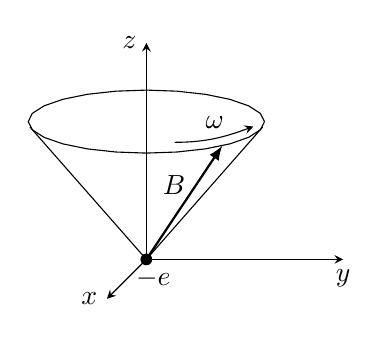
\begin{tikzpicture}
\pgfmathsetmacro{\a}{1.5}
\pgfmathsetmacro{\m}{0.7}
\pgfmathsetmacro{\b}{0.4}
\pgfmathsetmacro{\c}{1.75}
\draw[-stealth] (0,0) node[circle, fill=black,inner sep=1.5pt]{} node[below,xshift=0.25em]{$-e$} -- (-0.5,-0.5) node[left]{$x$};
\draw[-stealth] (0,0) -- (2.5,0) node[below]{$y$};
\draw[-stealth] (0,0) -- (0,2.75) node[left]{$z$};
\draw[] plot[domain=0:360] ({\a*cos(\x)},{\c+\b*sin(\x)});
%\draw[-stealth] plot[domain=290:350] ({\m*\a*cos(\x)},{\c+\m*\b*sin(\x)}) node[above left,yshift=-0.25em]{$\omega$};
\draw[thick, -latex] (0,0) -- ({\a*cos(310)},{\c+\b*sin(310)}) node[pos=0.65,left]{$\kvec{B}$};
\draw[] (0,0) -- ({\a*cos(190)},{\c+\b*sin(190)});
\draw[] (0,0) -- ({\a*cos(350)},{\c+\b*sin(350)});
\draw[-stealth] ({\m*\a*cos(290)},{\c+\m*\b*sin(290)})  to [out=0,in=-160] node[pos=0.5,above]{$\omega$} ++ (1,0.2);
\end{tikzpicture}
\caption{مقناطیسی میدان  زاویائی  سمتی رفتار \عددی{\omega} سے مخروطی راہ جھاڑتا ہے (مساوات \حوالہء{10.24})۔   }
\label{شکل_حرارت_نا_گزر_مخروطی_راہ_جھاڑنا}
\end{figure}


اس کا ہيملٹنی مساوات 4.158 درج ذیل ہوگا 
\begin{gather}
\begin{aligned}
H(t) &= \frac{e}{m} \kvec{B} \cdot \kvec{S} = \frac{e \hslash \beta_0}{2m} [\sin \alpha \cos(\omega t) \sigma_x + \sin \alpha \sin(\omega t) \sigma_y + \cos \alpha \sigma_z] \\
&= \frac{\hslash \omega_1}{2}
\begin{pmatrix}
\cos \alpha& e^{-i\omega t}\sin \alpha\\
e^{i\omega t}\sin\alpha& -\cos\alpha
\end{pmatrix} 
\end{aligned}
\end{gather}
جہاں \عددی{\omega_0} درج ذیل ہیں 
\begin{align}
\omega_1 \equiv \frac{e \beta_0}{m}
\end{align}
ہيملٹنی \عددی{H(t)} کے معمول شدہ امتیازی چکر کار  \عددی{\chi_+} اور \عددی{\chi_-} درج ذیل ہیں۔
\begin{align}
\chi_+ (t) &= 
\begin{pmatrix}
\cos(\alpha/2) \\
e^{i \omega t} \sin(\alpha/2)
\end{pmatrix}\\
\chi_{-} (t) &= 
\begin{pmatrix}
e^{-i \omega t} \sin(\alpha/2) \\
- \cos(\alpha/2)
\end{pmatrix}
\end{align}
جو \عددی{
\kvec{B} (t)
} کے لمحاتی رخ کے ساتھ ہما چکر اور خلاف چکر کو ظاہر کرتے ہیں سوال 4.30 دیکھیں ان کے مطابقتی امتیازی اقدار درج ذیل ہونگے 
\begin{align}
E \pm = \pm \frac{\hslash \omega_1}{2}
\end{align}
فرض کریں \عددی{
\kvec{B} (0)
} کے ہمراہ الیکٹران حمہ میدان صورت سے آغاز کرتا ہے 
\begin{align}
\chi (0) = 
\begin{pmatrix} 
\cos(\alpha/2) \\
\sin(\alpha/2)
\end{pmatrix}
\end{align}
تابع وقت شروڈنگر مساوات کا بلکل ٹھیک حل درج ذیل ہوگا سوال 10.2
\begin{align}
\chi (t) = 
\begin{pmatrix}
[\cos(\lambda t/2) - i \frac{(\omega_1 - \omega)}{\lambda} \sin(\lambda t/2)] \cos(alpha/2) e^{- i \omega t/2} \\
[\cos(\lambda t/2) - i \frac{(\omega_1 + \omega)}{\lambda} \sin(\lambda t/2)] \cos(alpha/2) e^{+ i \omega t/2}
\end{pmatrix}
\end{align}
جہاں \عددی{\lambda} درج ذیل 
\begin{align}
\lambda \equiv \sqrt{\omega^2 + \omega_1^2 - 2 \omega \omega_1 \cos \alpha}
\end{align}
جسے \عددی{\chi_{+}} اور \عددی{\chi_{-}} کا خطی مجموعہ لکھا جا سکتا ہے 
\begin{multline}
\chi (t) = \big [ \cos\big ( \frac{\lambda t}{2} \big ) - i \frac{(\omega_1 - \omega \cos \alpha)}{\lambda} \sin\big ( \frac{\lambda t}{2} \big ) \big ] e^{- i \omega t/2} \chi_{+} (t) \\
+ i \big [ \frac{\omega}{\lambda} \sin \alpha \sin \big ( \frac{\lambda t}{2} \big ) \big ] e^{+ i \omega t/2} \chi_- (t)
\end{multline}
ظاہر ہے کہ \عددی{\kvec{B}} کے موجودہ رخ کے لحاظ سے خلاف میدان کو تحویل کا ٹھیک ٹھیک احتمال درج ذیل ہوگا 
\begin{align}
\abs{\langle \chi (t) | \chi_{-} (t) \rangle}^2 = \big [ \frac{\omega}{\lambda} \sin \alpha \sin \big ( \frac{\lambda t}{2} \big ) \big ]^2
\end{align}
مسئلہ حرارت نہ گزر کہتا ہے کہ \عددی{
T_e \gg T_i
} کی تحدیدی صورت میں تحویلی احتمال صفر کو پہنچے گا جہاں ہيملٹنی میں تبدیلی کو درکار امتیازی وقت \عددی{T_e} ہے جو موجودہ صورت میں \عددی{1/\omega} ہوگا اور تفاعل موج میں تبدیلی کے لیے درکار امتیازی وقت \عددی{T_i} ہوگا جو موجودہ صورت میں \عددی{
\hslash / (E_{+} - E_{-} = 1/\omega_1)
} ہوگا یو حرارت نہ گزر تخمین سے مراد \عددی{\omega \ll \omega_1} ہوگا غیر مضطرب تفاعلات موج کے دور کے لحاظ سے میدان آہستہ گھومتا ہے حرارت نہ گزر صورت \عددی{
\lambda \cong \omega_1
} میں درج ذیل ہوگا ۔
\begin{align}
\abs{\langle \chi (t) | \chi_{-} (t) \rangle}^2 \cong \big [ \frac{\omega}{\omega_1} \sin \alpha \sin \big ( \frac{\lambda t}{2} \big ) \big ]^2 \to 0
\end{align}
%
\begin{figure}
\centering
\pgfmathsetmacro{\a}{1.1}
\pgfmathsetmacro{\b}{sin(deg(\a))^2}
\begin{tikzpicture}[declare function={f(\x)=(sin(deg(\a))*sin(\x/2))^2;}]
\begin{axis}[axis lines=middle,xlabel={$t$},ylabel={$\abs{\langle\chi(t)|\chi_{-}(t)\rangle}^2$}, xtick={360,720,1080,1440}, xticklabels={$2\pi/\lambda$,$4\pi/\lambda$,$6\pi/\lambda$,$8\pi/\lambda$}, ytick={\b,1}, yticklabels={$(\tfrac{\omega\sin\alpha}{\lambda})^2$,$1$}, xlabel style={at={(current axis.right of origin)}, anchor={north}} ,ylabel style={at={(current axis.above origin)},anchor=west},enlargelimits]
\addplot [thick,domain=0:1500,samples=500] {f(x)};
\addplot [dashed] coordinates{(0,1)(1500,1)};
\addplot [dashed] coordinates{(0,\b)(1500,\b)};
\end{axis}
\end{tikzpicture}
\caption{غیر حرارت نا گزر صورت   \عددی{(\omega\gg\omega_1)}   میں تحویلی  احتمال  (مساوات \حوالہء{10.34})۔}
\label{شکل_حرارت_نا_گزر_تحویلی_احتمال}
\end{figure}

جیسا ہم پہلے ذکر کر چکے مقناطیسی میدان الیکٹران کو ہاتھ سے پکڑ کر یو گھماتا ہے کے الیکٹران کا چکر ہر لمحہ پر \عددی{\kvec{B}} کہ رخ ہو اس کے برعکس \عددی{
\omega \gg \omega_1
} کی صورت میں \عددی{
\lambda \cong \omega
} ہوگا اور نظام ہم میدان اور خلاف میدان صورتوں کے بیچ ٹپکیاں کھائے گا  (شکل \حوالہ{شکل_حرارت_نا_گزر_تحویلی_احتمال})۔
\انتہا{مثال}
\ابتدا{سوال}
تصدیق کیجئے گا کہ مساوات 10.25 کی ہيملٹنی کیلئے مساوات 10.31 تابع وقت شروڈنگر مساوات کو مطمئن کرتی ہے ساتھ ہی مساوات 10.33 کی تصدیق کریں اور دکھائیں کے عددی سروں کے مربّعوں کا مجموعہ ایک ہوگا جو معمول زنی کی شرط ہے 
\انتہا{سوال}
%=========================

\حصہ{ہیّت بيری}
\جزوحصہ{گرگٹی عمل}
آئے حصہ 10.1.1 میں مستعمل کامل ہے رگڑھ لتکن جس کے چبوترا کو ایک مقام سے دوسری مقام منتقل کیا جاتا ہوں پر دوبارہ نظر ڈالتے ہیں جسے استعمال کرتے ہوئے حرارت نہ گزر عمل کا تصور اخذ کیا گیا میں نے دھاوا کیا تھا کہ جب تک چبوترا کی حرکت اتنی  رقاص  کے دوری عرصہ کے لحاظ سے اتنی آہستہ ہو کے  رقاص  کی نمایاں حرکت کے دوران  رقاص  بہت ساری ارتعاش کرتا ہوں یہ اسی مستوئی میں یا اس کے متوازی مستوئی میں اسی  حیطہ اور اسی تعدد کے ساتھ جھومتا رہے گا۔
\begin{figure}
\centering
\pgfmathsetmacro{\r}{2}
\pgfmathsetmacro{\a}{40}
\pgfmathsetmacro{\b}{180-\a}
\begin{tikzpicture}
\draw[thick] (0,0) circle (\r);
\draw[thick] (-\r,0) to [out=-\a,in=-180] coordinate [pos=0.35] (tae) coordinate[pos=0.25](ta) (0,-0.75) to [out=0,in=-\b] coordinate [pos=0.65] (tbe) coordinate[pos=0.75] (tb) (\r,0);
\draw[thick] (ta) to [out=80,in=-150] node[pos=0.5,circle,fill=black,inner sep=1.5pt]{}coordinate[pos=0.5](kswabi) coordinate [pos=0.85](ka) coordinate [pos=0.1](kc) (0,\r);
\draw(kswabi)node[pin={-30:{\RL{صوابی}}}]{};
\draw[thick] (tb) to [out=100,in=-30] coordinate [pos=0.85](kb) coordinate [pos=0.1](kd) (0,\r);
\draw[-stealth] (-0.5,-0.75+0.2) to [out=-10,in=-170] (0.5,-0.75+0.2);
\draw[] (0,-0.75) node[below]{\RL{ارضی خط استوا}};
\draw[stealth-] ($(ta)+(-0.15,0.4)$) to [out=80,in=-110] ++ (0.15,0.5);
\draw[-stealth] ($(tb)+(0.15,0.4)$) to [out=100,in=-70] ++ (-0.15,0.5);
\draw[] (ka) to [out=-30,in=-150] node[pos=0.5,below]{$\theta$} (kb);
\RightAngle{(kc)}{(ta)}{(tae)}
\RightAngle{(kd)}{(tb)}{(tbe)}
\draw[] (0,\r+0.75) node[circle,fill=black,inner sep=1.5pt]{} --++ (0.2,-0.4) coordinate[pos=0.9](penb) node[pos=0.5,right]{\RL{رقاص}};
\draw[] (0,\r+0.75)  --++ (-0.3,-0.5) coordinate[pos=0.9](pena);
\draw[stealth-stealth] (pena) to [out=10,in=-150] (penb);
\end{tikzpicture}
\caption{سطح زمین پر رقاص کی حرارت ناگزر منتقلی۔}
\label{شکل_حرارت_نا_گزر_سطح_زمین_منتقل}
\end{figure}



 لیکن اگر میں اس کامل  رقاص  کو شمالی قطب پر لے جا کر مثلا صوابی شہر کے رخ جھولا دوں  (شکل \حوالہ{شکل_حرارت_نا_گزر_سطح_زمین_منتقل}) فی الحال تصور کریں کے دنیا گھوم نہیں رہی ہے میں اس کو بہت آہستہ آہستہ یعنی حرارت نہ گزر طریقہ سے صوابی سے گزرتے خط طول بلند پر چلتے ہوئے عرضی خط استوا تک پہنچتا ہوں یہاں پہنچ کر یہ شمال و جنوب جھولے گا میں اس کو عرضی خط استوا پر کچھ فاصلہ دور تک لے جاتا ہوں  رقاص  ابھی بھی شمال و جنوب جھولتا ہے آخر میں میں اس نئی خط طول بلند پر چلتے ہوئے چبوترا کو شمالی قطب منتقل کرتا ہوں آپ دیکھ سکتے ہیں کے  رقاص  اسی مستوی میں اب نہیں جھولے گا جہاں سے اس نے آغاز کیا یقینا نئی مستوی اور پرانے مستوی کے بیچ زاویہ \عددی{\Theta} پایا جاتا ہے جہاں جنوب کی طرف چلتے ہوئے اور شمال کی طرف چلتے ہوئے دو خط طول بلند کے بیچ زاویہ \عددی{\Theta} ہے ہم دیکھتے ہیں کہ جس راہ پر میں چبوترا اٹھا کر چلتا رہا وہ راہ زمین کے مرکز پر ٹھوس زاویہ \عددی{\Omega} بناتی ہے یہ راہ شمالی نصف کرہ کا \عددی{
\Theta /2\pi
} حصہ گھیرتی ہے لہذا اس کا رقبہ \عددی{
A = (1/2)(\Theta/2\pi) 4\pi R^2 = \Theta R^2 
} ہوگا جہاں \عددی{ R} زمین کا رداس ہے یوں درج ذیل ہوگا ۔
\begin{align}
\Theta = A/R^2 \equiv \Omega
\end{align}
جو اس نتیجہ کو نہایت عمدگی کے ساتھ پیش کرتا ہے اور جو راہ کی شکل و صورت پر منحصر نہیں ہے  (شکل \حوالہ{شکل_حرارت_نا_گزر_کرہ_پر_ٹھوس_زاویہ})۔

\begin{figure}
\centering
\pgfmathsetmacro{\r}{2}
\begin{tikzpicture}
%\draw[thick] (-\r,-\r) grid (\r,\r);
%\draw[gray, step=0.1, thin] (-\r,-\r) grid (\r,\r);
\draw[thick] (0,0) circle (\r);
\draw[smooth, shading angle=130, ->-=0.15, ->-=0.5, ->-=0.65, ->-=0.85] plot [smooth] coordinates {(-1,1.25) (-1.25,1.25) (-1.75,0.5) (-1.25,0.75) (-0.25,0.5) (0.25,0.75) (-0.25,1)}--cycle;
\draw[] (-0.25,0.5) -- (0,0);
\draw[] (0.25,0.75) -- (0,0)coordinate[pos=0.5](kbb);
\draw[] (-1.75,0.5) -- (0,0)coordinate[pos=0.5](kaa);
\draw[stealth-] (kaa) to [out=-100,in=130] (0,-0.5);
\draw[stealth-] (kbb) to [out=-30,in=30] (0,-0.5)node[fill=white]{$\Omega$};
\end{tikzpicture}
\caption{کرہ پر اختیاری راہ، ٹھوس زاویہ \عددی{\Omega} بناتا ہے۔}
\label{شکل_حرارت_نا_گزر_کرہ_پر_ٹھوس_زاویہ}
\end{figure}


 کرہ کی سطح پر ایک بند راہ پر چلتے ہوئے حرارت نہ گزر منتقلی کی ایک مثال فوکالٹ  رقاص  ہے جہاں چبوترا کو اٹھا کر چلنے کی بجائے زمین کے گھومنے کو یہ کام سونپا جاتا ہے خط عرض بلد \عددی{\theta_0} درج ذیل ٹھوس زاویہ بناتا ہے  (شکل   \حوالہ{شکل_حرارت_نا_گزر_فوقو_رقاص_ایک_دن})۔ 
\begin{align}
\Omega = \int \sin \theta \dif \theta \dif \phi = 2\pi (- \cos \theta)_0^{\theta_0} = 2 \pi (1 - \cos \theta_0)
\end{align}
%
\begin{figure}
\centering
\pgfmathsetmacro{\r}{2}
\pgfmathsetmacro{\a}{0.8*\r}
\pgfmathsetmacro{\t}{90-acos(\a/\r)}
\pgfmathsetmacro{\b}{sqrt(\r^2-\a^2)}
\begin{tikzpicture}
\draw[] (0,0) circle (\r);
\draw[thick] (0,\a-0.05) circle (\b cm and 0.2cm);
\draw[] (0,0) node[fill=black,circle, inner sep=1.5pt]{} --++ (52.4:\r-0.1);
\draw[-stealth] (0,-0.25) -- (0,2.5) node[left]{$z$};
\draw[] ([shift={(90:0.5)}]0,0) arc (90:52.4:0.5) node[pos=0.5,above,xshift=0.25em]{$\theta_0$};
\end{tikzpicture}
\caption{ایک دن کے دوران، فوقو رقاص کی راہ۔}
\label{شکل_حرارت_نا_گزر_فوقو_رقاص_ایک_دن}
\end{figure}



زمین کے لحاظ سے جو اس دوران \عددی{2\pi} زاویہ گھوم چکا ہوگا فوکالٹ   رقاص   کی روزانہ استقبالی حرکت  \عددی{
2\pi \cos \theta_0
} ہوگی اس نتیجہ کو عموما گھومتی حوالہ چوکھٹ پر كوليولس کوتو کی اثر سے حاصل کیا جاتا ہے لیکن یہاں یہ خالصتا جومٹرئے مفہوم پیش کرتا ہے ایسا نظام جو بند راہ پر چل کے واپس ابتدائی نکتہ پہنچ کر اپنی ابتدائی حال میں نہیں لوٹتا غیر ہما قوائد نظام کہلاتا ہے یہاں ضروری نہیں کے راہ پر چلنے سے مراد حرکت دینا ہو اس سے مراد صرف اتنا ہے کہ نظام کی مقدار معلوم قیمتوں کو یوں تبدیل کیا جاتا ہے کہ آخر کار ان کی قیمتیں وہی ہوں جو ابتدا میں تھی غیر ہما قوائد نظام ہر جگہ پائے جاتے ہیں ایک لحاظ سے ہر چکر دار انجن غیر ہما قوائد اعلی ہے ہر ایک پیرا کے اختتام تک گاڑی آگے حرکت کر چکی ہوگی یا کوئی وزن اٹھایا گیا ہوگا وغیرہ وغیرہ اگلے حصہ میں میں غیر ہما قواعد اعمالوں کی کوانٹم میکانیات پر غور کروں گا ہم نے دیکھنا ہوگا کے ہيملٹنی کے مقدار معلوم مقداروں کو کسی بند راہ پر حرارت نہ گزر پیرا دینے سے احتتامی حال کس طرح ابتدائی حال سے مختلف ہوگا 
%==========================
\جزوحصہ{ہندسی ہیّت}
میں نے حصہ 10.1.2 میں دکھایا کے ایک ذرا جو \عددی{H(0)} کے \عددی{n} وی امتیازی حال سے آغاز کرتا ہو حرارت نہ گزر حالات میں تابع وقت ہيتى جزو ضربی کے علاوہ \عددی{H(t)} کی \عددی{n} وی امتیازی حال میں ہوگا بالخصوص اس کا تفاعل موج مساوات 10.23 درج ذیل ہوگا 
\begin{align}
\Psi_n (t) = e^{i[\theta_n (t) + \gamma_n (t)]} \psi_n (t)
\end{align} 
جہاں 
\begin{align}
\theta_n (t) \equiv - \frac{1}{\hslash} \int_0^t E_n (t') \dif t'
\end{align}
 حرکی ہیّت ہے جو تابع وقت تفاعل \عددی{E_n} کی صورت کے لیے جزو ضربی \عددی{
e^{(- i E_n t/\hslash)}
} کو عمومیت دیتا ہے اور درج ذیل ہندسی ہیّت کہلاتا ہے
\begin{align}
\gamma_n(t)\equiv \int_0^t \langle \psi_n(t')|\frac{\partial}{\partial t'}\psi_n(t')\rangle \dif t'
\end{align}

 چونکہ اب ہيملٹنی میں کوئی ایسا مقدار معلوم \عددی{R(t)} پایا جاتا ہے جو وقت کے ساتھ تبدیل ہوتا ہے لہذا \عددی{
\psi_n (t)
} وقت \عددی{ t} کا تابع ہوگا سوال 10.1 میں پھیلتے ہوئے چکور کنواں کی چوڑائی \عددی{R(t)} ہوگی یوں درج ذیل ہوگا 
\begin{align}
\frac{\partial \psi_n}{\partial t} = \frac{\partial \psi_n}{\partial \kvec{R}} \frac{\dif \kvec{R}}{\dif t}
\end{align}
لہذا درج ذیل ہوگا 
\begin{align}
\gamma_n (t) = i \int_0^t \langle \psi_n | \frac{\partial \psi_n}{\partial R} \rangle \frac{\dif R}{\dif t'} \dif t' = i \int_{R_i}^{R_f} \langle \psi_n | \frac{\partial \psi_n}{\partial R} \dif R 
\end{align}
جہاں \عددی{R_i} اور \عددی{R_f} مقدار معلوم \عددی{R_t} کے بالترتیب ابتدائی اور اختتامی قیمتیں ہوں گی بالخصوص اگر کچھ دیر \عددی{ T} بعد ہیملٹنی واپس اپنی ابتدائی روپ اختیار کرے تب \عددی{
R_f = R_i
} لہذا \عددی{
\gamma_n (T) = 0
} ہوگا جو زیادہ دلچسپ صورت حال نہیں ہے

 میں نے مساوات 10.41 میں فرض کیا کہ ہيملٹنی میں صرف ایک مقدار معلوم ایسا ہے جو تبدیل ہوتا ہو فرض کریں \عددی{N} عدد مقدار معلوم \عددی{R_1 (t)}،  \عددی{R_2 (t)}، \عددی{\dotsc}، \عددی{R_N (t)} تبدیل ہوتے ہوں تب درج ذیل ہوگا 
\begin{align}
\frac{\partial \psi_n}{\partial t} = \frac{\partial \psi_n}{\partial R_1} \frac{\dif R_1}{\dif t} + \frac{\partial \psi_n}{\partial R_2} \frac{\dif R_2}{\dif t} + \cdots + \frac{\partial \psi_n}{\partial R_N} \frac{\dif R_N}{\dif t} = (\nabla_R \psi_n) \cdot \frac{\dif \kvec{R}}{\dif t}
\end{align} 
جہاں \عددی{
\kvec{R} \equiv (R_1, R_2, \dotsc , R_N) 
} ہے اور \عددی{\nabla_R} ان مقدار معلوم کے لحاظ سے ڈھلوان ہے اس مرتبہ درج ذیل ہوگا 
\begin{align}
\gamma_n (t) = i \int_{\kvec{R}_i}^{\kvec{R}_f} \langle \psi_n | \nabla_R \psi_n \rangle \cdot \dif \kvec{R}
\end{align}
اور اگر وقت \عددی{ T} کے بعد ہیملٹنی واپس اپنی اصل روپ اختیار کرتا ہوں تب کل ہندسى ہیّتی تبدیلی درج ذیل ہوگی 
\begin{align}
\gamma_n (T) = i \oint \langle \psi_n | \nabla_R \psi_n \rangle \cdot \dif \kvec{R}
\end{align}
یہ مقدار معلوم فضا میں ایک بند راہ پر لکیری تکمل ہے جو عموما غیر صفر ہوگا مساوات 10.45 کو پہلی مرتبہ  \سن{ 1984}  میں میکائل بیری نے حاصل کیا اور یوں \عددی{
\gamma_n (T)
} ہیّت بیری کہلاتا ہے دھیان رہے ہیں کہ جب تک تبدیلی اتنی آہستہ ہو کہ قیاس حرارت نا گزر کے شرائط مطمئن ہوتے ہوں \عددی{
\gamma_n (T)
} کی قیمت صرف اس راہ پر منحصر ہوگی جس پر چلا جائے نا کہ راہ پر چلنے کی رفتار پر اس کے برعکس مجموعی حرکتی ہیّت 
\begin{align*}
\theta_n (T) = - \frac{1}{\hslash} \int_0^T E_n (t') \dif t'
\end{align*}
گزرے ہوئے وقت کا تابع ہوگا

 ہم اس سوچ کے عادی ہیں کہ تفاعل موج کا ہیّت کچھ بھی ہو سکتا ہے اور طبی مقداروں میں جہاں \عددی{
\abs{\Psi}^2
} پایا جاتا ہے ہیّتی جزو ضرب کٹ جاتا ہے اسی لیے عموما لوگوں کا خیال تھا کہ ہندسی ہیّت کی کوئی طبی اہمیت نہیں پائی جاتی ہے آخر \عددی{\psi_n (t)} کا ہیّت بھی اختیاری ہے یہ جناب بیری کی دور اندیشی ہے کہ انہوں نے اس حقیقت کو پہچانا کہ ہيملٹنی کو کسی بند دائرے پر لے جاتے ہوئے واپس اپنی اصل روپ میں لانے سے ابتدائی اور احتتامی  ہیّت کے بیچ فاصلہ غیر اختیاری ہوگا جسے حقیقتا ناکا جا سکتا ہے مثال کے طور پر زراعت جو تمام حال \عددی{\Psi} میں ہوں کی ایک شعاع کو دو حصوں میں تقسیم کرکے صرف ایک حصے کو حرارت نہ گزر تبدیل ہوتے مخفیا سے گزارا جاتا ہے دونوں حصوں کو دوبارہ اکھٹا کرنے سے مجموعی تفاعل موج درج ذیل روپ کا حاصل ہوگا 
\begin{align}
\Psi = \frac{1}{2} \Psi_0 + \frac{1}{2} \Psi_0 e^{i \Gamma}
\end{align}
جہاں سیدھی پہنچتی شعاع کا تفاعل موج \عددی{\Psi_0} ہے اور متغیر \عددی{H} کی بنا شعاع کا اضافی ہیّت \عددی{\Gamma} ہے جس کا کچھ حصہ ہرکی اور کچھ حصہ ہندسی ہوگا اس صورت میں درج ذیل ہوگا 
\begin{align}
\abs{\Psi}^2 &= \frac{1}{4} \abs{\Psi_0}^2 \big ( 1 + e^{i \Gamma} \big ) \big ( 1 + e^{- i \Gamma} \big ) \\
&= \frac{1}{2} \abs{\Psi_0}^2 (1 + \cos \Gamma) = \abs{\Psi_0}^2 \cos^2 (\Gamma/2)
\end{align}
یوں تعمیلی مداخلت اور تباہ کن مداخلت نکات جہاں \عددی{\Gamma} کی قیمت \عددی{\pi} کی بالترتیب جفت اور طاق مضرب ہوگی کو دیکھ کر ہم \عددی{\Gamma} کی پیمائش کر سکتے ہیں بیری اور دیگر مصنفین کو شبہ تھا کہ زیادہ بڑی ہرکی ہیّت کی موجودگی میں ہندسی ہيت نظر نہیں آئے گی لیکن انہیں علیحدہ کرنا ممکن ثابت ہوا ہے تین آبادی مقدار معلوم فضا \عددی{
\kvec{R} = (R_1, R_2, R_3)
} کی صورت میں کلیاں بیری مساوات 10.45 سمتی مخفیہ \عددی{\kvec{A}} کی صورت میں مقناطیسی بہاؤ کہ کلیہ کا یاد دلاتی ہے سطح \عددی{S} جس کی سرحد منحنی \عددی{ C} ہو سے درج ذیل
 بہاؤ گزرتا ہے  (شکل \حوالہ{شکل_حرارت_نا_گزر_مقناطیسی_بہاو})۔ 
\begin{align}
\Phi \equiv \int_S \kvec{B} \cdot \dif \kvec{a}
\end{align}

\begin{figure}
\centering
\begin{tikzpicture}[scale=2]
%\draw[thick] (0,0) grid (3,2.5);
%\draw[thin,step=0.1] (0,0) grid (3,2.5);
\draw[thick,fill=lgray] plot[smooth cycle] coordinates{(0,1)(1,0.5)(2,1) (1.5,2)(0.5,1.75)};
\draw[] (0,1) node[left]{$C$};
\draw[fill=white] (0.5,1.25) --++ (0.3,0) --++ (0.1,0.2) --++ (-0.3,0) -- cycle; 
\draw[-latex, thick](0.7,1.35) --++ (0,1) node[left]{$\dif\kvec{a}$};
\draw[fill=white] (0.5,1) circle (3pt and 2pt);
\draw[fill=white] (1,0.7) circle (3pt and 2pt);
\draw[fill=white] (1.5,1) circle (3pt and 2pt);
\draw[fill=white] (1.25,1.5) circle (3pt and 2pt);
\draw[-stealth](0.5,1) to [out=90,in=-45] ++ (-0.5,1)node[left]{$\kvec{B}$};
\draw[-stealth](1,0.7) to [out=10,in=135] ++ (1,-0.5)node[right]{$\kvec{B}$};
\draw[-stealth](1.5,1) to [out=50,in=-160] ++ (1,0.5)node[right]{$\kvec{B}$};
\draw[-stealth](1.25,1.5) to [out=80,in=-170] ++ (1,0.5)node[right]{$\kvec{B}$};
\draw[] (0.6,0.8) to [out=-135,in=0] ++ (-0.5,-0.5) node[left]{$S$};
\end{tikzpicture}
\caption{بند  منحنی  \عددی{C} کے بیچ سطح \عددی{S} سے گزرتا مقناطیسی بہاو۔}
\label{شکل_حرارت_نا_گزر_مقناطیسی_بہاو}
\end{figure}


مقناطیسی میدان کو سمتی مخفیہ کئی روپ میں \عددی{
(\kvec{B} = \nabla \times \kvec{A})
} لکھ کر مسئلہ سٹوکس کی اطلاق سے درج ذیل حاصل ہوگا 
\begin{align}
\Phi = \int_S (\nabla \times \kvec{A}) \cdot \dif \kvec{a} = \oint_C \kvec{A} \cdot \dif \kvec{r}
\end{align}
یوں مقدار معلوم فضا میں بند راہ کے اندر سے مقناطیسی میدان کے بہاؤ 
\begin{align}
\kvec{``B"} = i \nabla_R \times \langle \psi_n | \nabla_R \psi_n \rangle
\end{align}
کو  ہيّت  بیری تصور کیا جا سکتا ہے دوسرے لفظوں میں تین آبادی صورت میں ہیّت بیری کو ایک سطحی تکمل کی صورت میں لکھا جا سکتا ہے 
\begin{align}
\gamma_n (T) = i \int [\nabla_R \times \langle \psi_n | \nabla_R \psi_n \rangle ] \cdot \dif \kvec{a}
\end{align}
مقناطیسی مماثلت کو کافی دور تک لے جایا جا سکتا ہے تاہم ہماری استعمال کے نقطہ نظر سے مساوات 10.51 محض \عددی{
\gamma_n (T)
} کو لکھنے کا دوسرا انداز ہے 
%==========================

\ابتدا{سوال}
\begin{enumerate}[a.]
\item
لامتناہی چکور کنواں کی چوڑائی  \عددی{w_1} سے بھڑ کر \عددی{w_2} ہونے کی صورت میں مساوات 10.42 استعمال کرتے ہوئے ہندسی تبدیلی ہیئت تلاش کریں 
\item
اگر وسعت مستقل شرح \عددی{
(\dif w / \dif t = v)
} سے بڑھے تب ہرکی تبدیلی ہیئت کیا ہوگی 
\item
اب اگر چوڑائی کم ہو واپس \عددی{w_1} ہوجاتی ہے تب اس ایک تیرے کا ہیّت بیری کیا ہوگا 
\end{enumerate}
\انتہا{سوال}
\ابتدا{سوال}
ڈیلٹا تفاعل کنواں مساوات 2.114 واحد ایک مقید حال مساوات 2.129 کا حامل ہے \عددی{\alpha} آہستہ آہستہ \عددی{\alpha_1} سے بڑھ کر \عددی{\alpha_2} ہوتا ہے ہندسی تبدیلی ہیئت کا حساب لگائیں اگر تبدیلی ایک مستقل شرح \عددی{
\dif \alpha / \dif t = c
} سے رونما ہو تب ہرکی تبدیلی ہیئت کیا ہوگا 
\انتہا{سوال}
\ابتدا{سوال}
دکھائی کے حقیقی \عددی{
\psi_n (t)
} کی صورت میں ہنسی ہیّت صفر ہوگا سوال 10.3 اور 10.4 اس کی مثالیں ہیں امتیازی تفاعل کے ساتھ ایک غیر ضروری لیکن قانونی طور پر بالکل جائز جزو ضربی ہیّت منسلک کریں \عددی{
\psi'_n (t) \equiv e^{i \Phi_n} \psi_n (t)
} جہاں \عددی{
\Phi_n (\kvec{R})
} ایک اختیاری حقیقی تفاعل ہے یقینا آپ غیر صفر ہندسی ہيت حاصل کریں گے لیکن دیکھنا یہ ہے کہ اسے مساوات 10.23 میں پر کرنے سے کیا ہوگا اور بند راہ پر صفر حاصل ہوگا سبق غیر صفر ہیّت بیری کی خاطر آپ کو ایک ہیملٹنی میں ایک سے زیادہ تابع وقت مقدار معلوم کی ضرورت ہوگی اور دو  ایسا ہیملٹنی درکار ہوگا جو غیر صفر مخلوط امتیازی تفاعلات دیتا ہوں 
\انتہا{سوال}
\ابتدا{مثال} 
ہیّت بیری کی کلاسیکی مثال ایک مستقل مقدار کی مقناطیسی میدان جس کی سمت تبدیل ہوتی ہو میں مبدا پر پڑا ہوا ایک الیکٹران ہے پہلے اس خصوصی صورت کو دیکھتے ہیں جس کا تجزیہ مثال 10.1 میں کیا گیا اور جس میں محور \عددی{z} کے ساتھ ایک اٹل زاویا \عددی{\alpha} بناتے ہوئے \عددی{
\kvec{B} (t)
} ایک مستقل زاویائی سمتی رفتار \عددی{\omega} سے استقبالی حرکت کرتا ہو میدان بھی کے ساتھ ساتھ ہم میدان الیکٹران کی صورت میں مساوات 10.33 ٹھیک ٹھیک حل دیتی ہے حرارت نہ گزر صورت \عددی{
\omega \ll \omega_1
} میں 
\begin{align}
\lambda = \omega_1 \sqrt{1 - 2 \frac{\omega}{\omega_1} \cos \alpha + \big ( \frac{w}{w_1} \big )^2 } \cong \omega_1 \big ( 1 - \frac{\omega}{\omega_1} \cos \alpha \big ) = \omega_1 - \omega \cos \alpha
\end{align}
ہوگا لہذا مساوات 10.33 درج ذیل روپ اختیار کرے گی 
\begin{multline}
\chi (t) \cong e^{- i \omega_1 t/2} e^{i (\omega \cos \alpha) t/2} e^{- i \omega t/2} \chi_+(t) \\
i \big [ \frac{\omega}{\omega_1} \sin \alpha \sin \big ( \frac{\omega_1 t}{2} \big ) \big ]e^{+ i \omega t/2} \chi_{-} (t)
\end{multline}
دوسرے جزو کو \عددی{
\omega/\omega_1 \to 0
} کی صورت میں رد کرتے ہوئے مساوات 10.23 کے مطابق نتیجہ حاصل ہوگا ہرکی ہیّت درج ذیل ہے 
\begin{align}
\theta + (t) = - \frac{1}{\hslash} \int_0^t E + (t') \dif t' = - \frac{\omega_1 t}{2}
\end{align}
جہاں مساوات 10.29 سے \عددی{
E_{+} = \hslash \omega_1 /2
} ہوگا لہذا ہندسی ہیّت درج ذیل ہوگی 
\begin{align}
\gamma + (t) = (\cos \alpha - 1) \frac{\omega t}{2}
\end{align}
ایک مکمل پیرا کے لیے \عددی{
T = 2\pi / \omega
} ہوگا لہذا ہیّت بیری درج ذیل ہوگی 
\begin{align}
\gamma + (T) = \pi (\cos \alpha - 1)
\end{align}

\begin{figure}
\centering
\begin{tikzpicture}
%\draw[thick] (0,0) grid (3,2.5);
%\draw[thin,step=0.1] (0,0) grid (3,2.5);
\draw[thick,fill=lgray,->-=0,->-=0.5] plot[smooth cycle] coordinates{(0,1)(1,0.5)(2,1) (1.5,2)(0.5,1.75)};
\draw[] (1.5,0.2) node[circle,fill=black,inner sep=1.5pt]{} circle (2);
\draw[-stealth, thick] (1.5,0.2) node[below]{$-e$} -- (1.9,0.85) node[pos=0.6,right]{$\kvec{B}$};
\end{tikzpicture}
\caption{مستقل  مقدار لیکن بدلتے رخ کا مقناطیسی میدان بند راہ پر چلتا ہے۔}
\label{شکل_حرارت_نا_گزر_مقناطیسی_میدان_بند_راہ}
\end{figure}

اب ایک زیادہ عمومی صورت پر غور کرتے ہیں جس میں مقناطیسی میدان سمتیہ کی نوک رداس \عددی{
r = B_0
} کی کراں کہ سطح ہر ایک اختیاری بند راہ پر چلتا ہے  (شکل  \حوالہ{شکل_حرارت_نا_گزر_مقناطیسی_میدان_بند_راہ})۔ میدان \عددی{
\kvec{B} (t)
} کے ساتھ ساتھ ہم میدان کو ظاہر کرنے والا امتیازی حال درج ذیل روپ کا ہوگا سوال 4.30 دیکھیں 
\begin{align}
\chi_{+} = 
\begin{pmatrix}
\cos (\theta/2) \\
e^{i \phi} \sin (\theta /2)
\end{pmatrix}
\end{align}
جہاں \عددی{\kvec{B}} کے دونوں کروی مہدد \عددی{\theta} اور \عددی{\pi} وقت کے تفاعلات ہیں کروی مہدد میں ڈھلواں درج ذیل ہوگا جیسے آپ جدول سے دیکھ سکتے ہیں 
\begin{align}
\nabla \chi_{+} &= \frac{\partial \chi_{+}}{\partial r} \hat{r} + \frac{1}{r} \frac{\partial \chi_{+}}{\partial \theta} \hat{\theta} + \frac{1}{r \sin \theta} \frac{\partial \chi_{+}}{\partial \phi} \hat{\phi} \\
&= \frac{1}{r} 
\begin{pmatrix}
- (1/2) \sin (\theta/2) \\
(1/2) e^{i \phi} \cos (\theta /2)
\end{pmatrix}
\hat{\theta} + \frac{1}{r \sin \theta}
\begin{pmatrix}
0 \\
i e^{i \phi} \sin (\theta /2)
\end{pmatrix} 
\hat{\phi}
\end{align}
یوں درج ذیل ہوگا 
\begin{align}
\langle \chi_{+} | \nabla \chi_{+} \rangle &= \frac{1}{2r} \big [ - \sin (\theta /2) \cos (\theta /2) \hat{\theta} + \sin (\theta /2) \cos (\theta / 2) \hat{\theta} + 2i \frac{\sin^2 (\theta /2)}{\sin \theta} \hat{\phi} \big ] \\
&= i \frac{\sin^2 (\theta /2)}{r \sin \theta} \hat{phi}
\end{align}
مساوات 10.51 کے لیے ہمیں اس مقدار کی گردش درکار ہوگی 
\begin{align}
\nabla \times \langle \chi_{+} | \nabla \chi_{+} \rangle = \frac{1}{r \sin \theta} \frac{\partial}{\partial \theta} \big [ \sin \theta \big ( \frac{i \sin^2 (\theta /2)}{r \sin \theta} \big ) \big ] \hat{r} = \frac{i}{2r^2} \hat{r}
\end{align}
یوں مساوات 10.51 کے تحت درج ذیل ہوگا 
\begin{align}
\gamma_{+} (T) = - \frac{1}{2} \int \frac{1}{r^2} \hat{r} \cdot \dif \kvec{a}
\end{align}
تکمل قرہ کی سطح پر اس رقبے پر لیا جائے گا جس کو \عددی{\kvec{B}} کی چھوٹی ایک پیرا میں گرتا ہو لہذا \عددی{
\dif \kvec{a} = r^2 \dif \Omega \hat{r}
} ہوگا جس کے تحت درج ذیل ہوگا 
\begin{align} 
\gamma_{+} (T) = - \frac{1}{2} \int \dif \Omega = - \frac{1}{2} \Omega
\end{align}
جہاں مبده پر ٹھوس زاویا \عددی{\Omega} ہے یہ ایک انتہائی سادہ نتیجہ ہے جو ہمیں اس کلاسیکی مسئلہ کی یاد دلاتا ہے جس سے ہم نے یہ تبصرہ شروع کیا یعنی زمین کی سطح پر ایک بند راہ پر ایک بلا رگڑ   رقاص   کی منتقلی اس نتیجہ کے تحت کسی اختیاری بند راہ پر ایک مقناطیس کی مدد سے الیکٹران کے چکر کو حرارت نہ گزر طریقے سے لے جانے سے کل ہندسی تبدیلی ہیئت مقناطیسی میدان سمتیہ کی چھوٹی سے حاصل ٹھوس زاویا کی منفی منفی بادا ہوگا مساوات 10.37 کو مد نظر رکھتے ہوئے یہ عمومی نتیجہ مساوات 10.56 کہ خصوصی نتیجہ کے مطابق ہے جیسا یقینا ہونا بھی چاہیے 
\انتہا{مثال}
\ابتدا{سوال}
ایک ذرہ جس کا چکر ایک ہو کے لئے مساوات 10.62 کا مماثل حاصل کریں جواب \عددی{- \Omega} ایک ذرہ جس کا چکر \عددی{s} ہو کے لیے نتیجہ \عددی{-s \Omega} 
\انتہا{سوال}

%===========================

 \جزوحصہ{اہارونو و بوہم اثر}\شناخت{حصہ_حرارت_نا_گزر_اہارونوبوہم_اثر}
کلاسیکی برقی حرکیات میں طبی مقداریں برقی اور مقناطیسی میدان ہیں؛ مخفیہ \عددی{\varphi} اور \عددی{
\kvec{A}
} بلاواسطہ ناقابل پیمائش ہیں 
\begin{align}
\kvec{E} = - \nabla \varphi - \frac{\partial \kvec{A}}{\partial t}, \quad \kvec{B} = \nabla \times \kvec{A}
\end{align}
میکسول مساوات اور قاعدہ لورنس قوت جیسے بنیادی قوانین مخفیا کا کوئی ذکر نہیں کرتے ہیں جو منطقی نقطہ نظر سے ایک نظریہ تشکیل دینے کے لیے کار آمد لیکن ویسے غیر ضروری ہیں یقینا ہم بغیر خوف و خطر ان مخفیات کو تبدیل کر سکتے ہیں 
\begin{align}
\varphi \to \varphi' = \varphi - \frac{\partial \Lambda}{\partial t}, \quad \kvec{A} \to \kvec{A}' = \kvec{A} + \nabla \Lambda
\end{align}
جہاں \عددی{\Lambda} مقام اور وقت کا کوئی بھی تفاعل ہو سکتا ہے اسے ماپ تبادلہ کہا جاتا ہے اور جیسا آپ مساوات 10.63 استعمال کرتے ہوئے دیکھ سکتے ہیں کہ اس کا میدانوں پر کوئی اثر نہیں ہوگا کوانٹم میکانیات میں مخفیہ زیادہ اہم کردار ادا کرتی ہے چونکہ ہیملٹنی کو \عددی{\varphi} اور \عددی{\kvec{A}} کی صورت میں نا کہ \عددی{\kvec{E}} اور \عددی{\kvec{B}} کی صورت میں بیان کیا جاتا ہے 
\begin{align}
H = \frac{1}{2m} \big ( \frac{\hslash}{i} \nabla - q \kvec{A} \big )^2 + q \varphi
\end{align}
بہرحال  زیر ماپ تبادلہ یہ نظریہ  غیر متغیر ہے سوال 4.61 دیکھیں اور بہت لمبہ  عرصہ کے لیے مانا گیا کہ  جن خطوں میں  \عددی{\kvec{E}} اور \عددی{\kvec{B}} صفر ہوں وہاں کسی قسم کا برقناطیسی اثر نہیں پایا جائے گا بالکل اسی طرح جس طرح کلاسیکی نظریہ میں ہوتا ہے لیکن \سن {1959} میں اہارونو اور بوہم نے دکھایا کہ اس خطہ میں بھی جہاں میدان صفر ہو سمتی مخفیہ حرکت پذیر باردار ذرا کے کوانٹائی رویہ پر اثر انداز ہوگا میں ایک سادہ مثال پیش کرنے کے بعد اہارونو و بوہم   اثر پر تبصرہ کے بعد اس کا تعلق ہیت بیری کے ساتھ پیش کروں گا۔


\begin{figure}
\centering
\pgfmathsetmacro{\a}{0.75}
\pgfmathsetmacro{\b}{5}
\pgfmathsetmacro{\d}{0.05}
\begin{tikzpicture}[]
\draw[] (0,0) -- (0,\b);
\draw[] (\a,0) -- (\a,\b);
\draw[] (0,0) to [out=-90,in=-90] ++ (\a,0);
\draw[] (\a/2,\b) circle (\a/2 and \a/6);
\foreach \kk in {0.2,0.6,...,\b}{
\draw[] (-\d,\kk) to [out=-160,in=-10] ++ (\a+2*\d,0.1);}
\path (-\d,3.8) to [out=-160,in=-10] coordinate[pos=0.5](tpa)coordinate[pos=0.55](tpb) ++ (\a+2*\d,0.1);
\draw[] (-\d,3.8) node[left]{$I$};
\draw[-stealth,thick] (\a/2,\b) --++ (0,0.75) node[right]{$\kvec{B}$};
\draw[-stealth, very thick] (tpa) -- (tpb);
\draw[] (\a/2,-0.3) --++ (0,-0.3) coordinate[pos=0.5](bota);
\draw[] (\a,-0.3) --++ (0,-0.3) coordinate[pos=0.5](botb);
\draw[-stealth] (bota) -- (botb) node[pos=0.5,below]{$a$};
\draw[very thick] plot[domain=105:435]({\a/2+2*cos(\x)},{\b/2+0.55*sin(\x)});
\draw  ({\a/2+2*cos(220)},{\b/2+0.55*sin(220)})node[circle,fill=black,inner sep=1.5pt]{}coordinate(kkk) node[below]{$q$};
\draw[-latex,shorten >=2pt](\a/2,\b/2)--(kkk) node[pos=0.75, above]{$b$};
\end{tikzpicture}
\caption{ایک دائرہ ، جس کے اندر سے ایک لمبا پیچواں برقی مقناطیس گزرتا ہو، پر ایک باردار ذرہ حرکت کرتا ہے۔ }
\label{شکل_حرارت_نا_گزر_پیچواں_دائرہ_حرکت}
\end{figure}

 فرض کریں ایک ذرا کو رداس \عددی{b} کے دائرہ پر رہنے کا پابند بنایا جائے اس دائرے کے محور پر رداس \عددی{
a < b
} کا ایک لمبا لچھا پایا جاتا ہے جس میں یک سمتی برقی رو \عددی{I} ہے  (شکل  \حوالہ{شکل_حرارت_نا_گزر_پیچواں_دائرہ_حرکت})   بہت لمبا لچھا کی صورت میں لچھے کے اندر مقناطیسی میدان یکساں ہوگا جبکہ بیرونی میدان صفر ہوگا تاہم لچھے کا بیرونی سمتی مخفیہ غیر صفر ہوگا یقینا موزوں ماپ شرط \عددی{
\nabla \cdot \kvec{A} = 0
} لیتے ہوئے درج ذیل ہوگا 
\begin{align}
\kvec{A} = \frac{\Phi}{2\pi r} \hat{\phi}, \quad (r > a)
\end{align}
جہاں \عددی{
\Phi = \pi a^2 B
} لچھے سے گزرتا ہوا  مقناطیسی بہاؤ ہوگا ساتھ ہی لچھا ازخود غیر باردار ہے لہذا غیر سمتی مخفیہ \عددی{\varphi} صفر ہے ایسی صورت میں ہیملٹنی مساوات 10.65درج ذیل روپ اختیار کرتی ہے 
\begin{align}
H = \frac{1}{2m} [- \hslash^2 \nabla^2 + q^2 A^2 + 2 i \hslash q \kvec{A} \cdot \nabla]
\end{align}
اب تفاعل موج صرف زاویہ اسّمت \عددی{
\phi (\theta = \pi/2, r = b) 
} پر منحصر ہے لہذا \عددی{
\nabla \to (\hat{phi} /b)(\dif / \dif \phi)
} ہوگا اور مساوات شروڈنگر درج ذیل لکھی جائے گی 
\begin{align}
\frac{1}{2m} \big [ - \frac{\hslash^2}{b^2} \frac{\dif^{\,2}}{\dif \phi^{\,2}} + \big ( \frac{q \Phi}{2 \pi b} \big )^2 + i \frac{h q \Phi}{\pi b^2} \frac{\dif}{\dif \phi} \big ] \psi (\phi) = E \psi (\phi)
\end{align}
یہ مستقل عددی سروں والی خطی تفرقی مساوات ہے
\begin{align}
\frac{\dif^{\,2} \psi}{\dif \phi^{\,2}} - 2i \beta \frac{\dif \psi}{\dif \phi} + \epsilon \psi = 0
\end{align}
جہاں درج ذیل ہیں
\begin{align}
\beta &\equiv \frac{q \Phi}{2 \pi \hslash}, && \epsilon \equiv \frac{2 m b ^2 E}{\hslash^2} - \beta^2
\end{align}
اس کے حل درج ذیل روپ کے ہونگے 
\begin{align}
\psi = Ae^{i \lambda \phi}
\end{align}
جہاں درج ذیل ہوگا 
\begin{align}
\lambda = \beta \pm \sqrt{ \beta^2 + \epsilon} = \beta \pm \frac{b}{\hslash} \sqrt{2 m E}
\end{align}
نقطہ \عددی{
\phi = 2\pi
} پر \عددی{\psi (\phi)} کی استمرار کی بنا \عددی{\lambda} عدد صحیح
\begin{align}
\beta \pm \frac{b}{\hslash} \sqrt{2m E} = n
\end{align} 
ہو گا جس سے درج ذیل حاصل ہوگا 
\begin{align} 
E_n = \frac{\hslash^2}{2m b^2} \big ( n - \frac{q \Phi}{2 \pi \hslash} \big )^2, \quad (n = 0, \pm 1, \pm 2, \dotsc)
\end{align}
لچها دائرے پر ذرا کی دوری انحطاط ختم کرتا ہے سوال 2.46 مثبت \عددی{n} جو لچھا میں رو کے رخ حرکت کرتے ہوئے ذرا کو ظاہر کرتا ہے \عددی{ q} مثبت لیتے ہوئے منفی \عددی{n} کے لحاظ سے جو مخالف رخ ذرا کو ظاہر کرتا ہے کے لحاظ سے نسبتا کم توانائی دیتا ہے زیادہ اہم بات یہ ہے کہ اجازتی توانائیوں کا دارومدار لچھے کے اندر میدان پر ہوگا اگرچہ اس مقام پر جہاں ذرا پایا جاتا ہے میدان صفر ہے زیادہ عمومی صورت پر غور کرنے کی خاطر فرض کریں ایک زرا ایسے خطہ میں حرکت کرتا ہے جہاں \عددی{\kvec{B}} ہے لہذا \عددی{
\nabla \times \kvec{A} = 0
} ہوگا تاہم \عددی{\kvec{A}} از خود غیر صفر ہے اگرچہ میں فرض کرتا ہوں کہ \عددی{\kvec{A}} ساکن ہے اس ترکیب کو تابع وقت مخفیا کے لئے عمومیت دی جا سکتی ہے مخفی توانائی \عددی{V} جس میں برقی حصہ \عددی{q \psi} شامل یا غیر شامل ہو سکتا ہے کی شروڈنگر مساوات 
\begin{align} 
\big [ \frac{1}{2m} \big ( \frac{\hslash}{i} \nabla - q \kvec{A} \big )^2 + V \big ] \Psi = i \hslash \frac{\partial \Psi}{\partial t}
\end{align}
کی سادہ روپ درج ذیل لکھ کر حاصل کی جاسکتی ہے 
\begin{align}
\Psi = e^{i g} \Psi'
\end{align}
جہاں \عددی{
g (\kvec{r})
} درج ذیل ہے 
\begin{align}
g (\kvec{r}) \equiv \frac{q}{\hslash} \int_{\mathcal{0}}^{\kvec{r}} \kvec{A} (\kvec{r}') \cdot \dif \kvec{r}'
\end{align}
اور \عددی{
\mathcal{0}
} کوئی بھی اختیاری نقطہ حوالہ ہے دھیان رہے کہ یہ تعریف صرف اس صورت بامعنی ہوگی جب پورا خطا میں \عددی{\nabla \times \kvec{A} = 0} ہو ورنہ لکیری تکمل \عددی{\mathcal{0}} سے \عددی{\kvec{r}} تک راہ پر منحصر ہوگا اور یوں \عددی{\kvec{r}} کا تفاعل نہیں ہوگا \عددی{\Psi'} کی صورت میں \عددی{\Psi} کا ڈلوان درج ذیل ہوگا 
\begin{align*}
\nabla \Psi = e^{i g} (i \nabla g) \Psi' + e^{\nabla \Psi'}
\end{align*}
لیکن \عددی{
\nabla g = (q/ \hslash) \kvec{A}
} کے برابر ہے لہذا 
\begin{align}
\big ( \frac{\hslash}{i} \nabla - q \kvec{A} \big ) \Psi = \frac{\hslash}{i} e^{i g} \nabla \Psi'
\end{align}
اور یوں درج ذیل ہوگا 
\begin{align}
\big ( \frac{\hslash}{i} \nabla - q \kvec{A} \big )^2 \Psi = - \hslash^2 e^{i g} \nabla^2 \Psi'
\end{align}
اس کو مساوات 10.75 میں پر کر کے مشترکہ جزو ضربی \عددی{e^{i g}} کو کاٹ کر درج ذیل ملتا ہے 
\begin{align}
- \frac{\hslash^2}{2m} \nabla^2 \Psi' + V \Psi' = i \hslash \frac{\partial \Psi'}{\partial t}
\end{align}
%
\begin{figure}
\centering
\pgfmathsetmacro{\a}{0.75}
\pgfmathsetmacro{\b}{5}
\pgfmathsetmacro{\d}{0.05}
\begin{tikzpicture}[]
\draw[very thick, ->-=0.1,->-=0.35,->-=0.75] (-3,\b/2+0.1) to [out=0,in=180]  (\a/2,\b/2+0.75) to [out=0,in=180] (3+\a,\b/2);
\draw[very thick, ->-=0.1,->-=0.35,->-=0.75,-stealth] (-3,\b/2-0.1) to [out=0,in=180]  (\a/2,\b/2-0.75) to [out=0,in=180] (3+\a,\b/2);
\fill[white] (-0.15,\b/2) rectangle (\a+0.15,\b/2+1);
\draw[] (-2,\b/2-0.25) node[pin={-130:{\RL{تقسیم شدہ شعاع}}}]{};
\draw[] (\a+2,\b/2-0.25) node[pin={-30:{\RL{دوبارہ ملاپ شعاع}}}]{};
\draw[] (0,0) -- (0,\b);
\draw[] (\a,0) -- (\a,\b);
\draw[] (0,0) to [out=-90,in=-90] ++ (\a,0);
\draw[] (\a/2,\b) circle (\a/2 and \a/6);
\foreach \kk in {0.2,0.6,...,\b}{
\draw[] (-\d,\kk) to [out=-160,in=-10] ++ (\a+2*\d,0.1);}
\path (-\d,3.8) to [out=-160,in=-10] coordinate[pos=0.5](tpa)coordinate[pos=0.55](tpb) ++ (\a+2*\d,0.1);
\draw[] (-\d,3.8) node[left]{$I$};
\draw[-stealth,thick] (\a/2,\b) --++ (0,0.75) node[right]{$\kvec{B}$};
\draw[-stealth, very thick] (tpa) -- (tpb);
\draw[](\a/2,0)node[below,yshift=-1em]{\RL{پیچواں برقی مقناطیس}};
\draw[-stealth] plot[domain=120:415]({\a/2+1*cos(\x)},{\b/2+0.25*sin(\x)});
\draw[] (\a/2+1,\b/2) node[right]{$\kvec{A}$};
\end{tikzpicture}
\caption{اہارانو و بوہم اثر: ایلکٹران شعاع تقسیم ہو کر  آدھا حصہ لمبے پیچواں برقی مقناطیس کے ایک طرف اور دوسرا حصہ دوسرے طرف سے گزرتا ہے۔ }
\label{شکل_حرارت_نا_گزر_اہارانووبوہم}
\end{figure}


بظاہر \عددی{\Psi'} بغیر \عددی{\kvec{A}} شروڈنگر مساوات کو مطمئن کرتا ہے مساوات 10.80 کا حل تلاش کرنے کے بعد بغیر گردش سمتی مخفیہ سے پیدا تصحیح کو شامل کرنا معمولی بات ہو گئی ہمیں صرف ہیتی جزو ضربی \عددی{e^{i g}} ساتھ منسلک کرنا ہوگا عہرانو اور بوہم نے ایک تجربہ تجویز کیا جس میں الیکٹران کی شعاع کو دو حصوں میں تقسیم کر کے لمبے لچھے کے دونوں اطراف سے گزار کر دوبارہ اکٹھا کیا جاتا ہے  (شکل   \حوالہ{شکل_حرارت_نا_گزر_اہارانووبوہم})  ان شعاعوں کو لمبے لچھا سے اتنا دور رکھا جاتا ہے جہاں \عددی{
\kvec{B} = 0
} ہو تاہم \عددی{\kvec{A}} جس سے مساوات 10.66 پیش کرتی ہے غیر صفر ہوگا اور دونوں اطراف \عددی{V} کی قیمت ایک دوسرے جیسی تصور کرتے ہوئے اختتامی نقطہ پر دونوں شعاعوں میں ہیتی فرق پایا جائے گا 
\begin{align}
g = \frac{q}{\hslash} \int \kvec{A} \cdot \dif \kvec{r} = \frac{q \Phi}{2 \pi \hslash} \int \big ( \frac{1}{r} \hat{\phi} \big ) \cdot (r \hat{\phi} \dif \phi ) = \pm \frac{q \Phi}{2 \hslash}
\end{align}
یہاں مثبت علامت ان الیکٹران کے لیے ہوگی جو لمبے لچھے میں \عددی{\kvec{A}} کے رخ حرکت کرتے ہیں دونوں شعاعوں کے بیچ ہیتی فرق اس مقناطیسی بہاؤ کے راست متناسب ہوگا جس سے ان کی راہ گیرتے ہیں 
\begin{align}
\text{\RL{ہیّتی فرق}}= \frac{q \Phi}{\hslash}
\end{align}
اس ہيتی ینتقل سے قابل پیمائش مداخلت مساوات 10.48 پیدا ہوتی ہے جس کی تجرباتی تصدیق چیمبرز اور ساتھی کر چکے ہیں اہارنو و بوہم اثر کو ہندسی ہیت کی ایک مثال تصور کی جا سکتی ہے فرض کریں مخفیہ \عددی{
 V(\kvec{r} - \kvec{R})
} ایک بار دار ذرا کو ایک ڈبہ میں رہنے کا پابند بناتا ہو جہاں ڈبے کا مرکز لمبے لچھے سے باہر نقطہ \عددی{\kvec{R}} پر ہے  ؛ شکل \حوالہ{شکل_حرارت_نا_گزر_مقید_ذرہ_ڈبیہ} دیکھیں۔     ہم کچھ ہی دیر میں اس ڈبہ کو لمبے لچھے کے گرد ایک پیرا دینگے لہذا \عددی{\kvec{R}} وقت کا تفاعل ہوگا تاہم ابھی اسے ایک غیر متغیر سمتیہ تصور کریں اس ہیملٹنی کے امتیازی تفاعلات درج ذیل تعین کرتی ہے 
\begin{align} 
\big \{ \frac{1}{2m} \big [ \frac{\hslash}{i} \nabla - q \kvec{A} (\kvec{r}) \big ]^2 + V (\kvec{r} - \kvec{R}) \big \} \psi_n = E_n \psi_n
\end{align}
%
\begin{figure}
\centering
\pgfmathsetmacro{\a}{0.75}
\pgfmathsetmacro{\b}{5}
\pgfmathsetmacro{\la}{1.5}
\pgfmathsetmacro{\lb}{1.5}
\pgfmathsetmacro{\lc}{1}
\begin{tikzpicture}[]
\draw[] (0,0) -- (0,\b);
\draw[] (\a,0) -- (\a,\b);
\draw[] (0,0) to [out=-90,in=-90] ++ (\a,0);
\draw[] (\a/2,\b) circle (\a/2 and \a/6);
\draw[] (3,3) coordinate(fa) --++ (\la,0) --++ (0, \lb) --++ (-\la,0) --++(0,-\lb);
\draw[] (3,3) ++ (\la,0) --++ (45:\lc) --++ (0,\lb) coordinate(fb) --++ (-\la, 0) --++ (45:-\lc);
\draw[] (3,3) ++ (\la,\lb) --++ (45:\lc);
\draw[] (\a/2,2) --++ (-0.2,-0.2);
\draw[] (\a/2,2) --++ (0.25,0);
\draw[] (\a/2,2) --++ (0,0.25);
\draw[-stealth,shorten >=2pt] (\a/2,2) -- ($(fa)!0.5!(fb)$) node[pos=0.5,above]{$\kvec{R}$} coordinate(tipa); 
\draw[-latex] (\a/2,2) -- ($(3+\la,3+\lb/5)+(45:\lc/3)$) node[pos=0.5,below]{$\kvec{r}$} coordinate(tipb); 
\draw[-stealth] (tipa)node[circle,fill=black,inner sep=1.5pt]{} -- (tipb) node[pos=0.25,pin={[pin distance=1.25cm,pin edge=-]30:{$(\kvec{r}-\kvec{R})$}}]{};
\end{tikzpicture}
\caption{مخفیہ \عددی{V(\kvec{r}-\kvec{R})} ایک ذرہ کوڈبیہ میں  مقید کیے ہوئے ہے۔}
\label{شکل_حرارت_نا_گزر_مقید_ذرہ_ڈبیہ}
\end{figure}

ہم اس طرز کی مساوات کو حل کرنا جانتے ہیں ہم
\begin{align}
\psi_n = e^{i g} \psi'_n
\end{align}
لیتے ہے جہاں درج ذیل ہوگا 
\begin{align}
g \equiv \frac{q}{\hslash} \int_{\kvec{R}}^{\kvec{r}} \kvec{A} (\kvec{r}') \cdot \dif (\kvec{r}')
\end{align}
اور \عددی{\psi'} اسی امتیازی قدر مساوات کو صرف اس صورت مطمئن کرے گا جب \عددی{\kvec{A} \to 0} ہو 
\begin{align}
\big [ - \frac{\hslash^2}{2m} \nabla^2 + V (\kvec{r} - \kvec{R}) \big ] \psi' = E_n \psi'_n
\end{align}
آپ نے دیکھا کہ \عددی{\psi'_n} ہٹاؤ \عددی{
\kvec{r} - \kvec{R}
} کا تفاعل ہے نہ کہ \عددی{\psi_n} کی طرح علیحدہ علیحدہ \عددی{\kvec{r}} اور \عددی{\kvec{R}} کا تفاعل آئیے اب اس ڈبہ کو لمبے لچھے کے گرد ایک پیرا دیتے ہیں یہاں اس عمل کا حرارت نہ گزر ہونے کے بھی ضرورت نہیں ہے ہیت بیری تعین کرنے کی خاطر ہمیں مقدار \عددی{
\langle \psi_n | \nabla \psi_n \rangle
} کی قیمت درکار ہوگی درج ذیل کی بنا 
\begin{align*}
\nabla_R \psi_n = \nabla_R [e^{i g} \psi'_n (\kvec{r} - \kvec{R})] = - \frac{q}{\hslash} \kvec{A} (\kvec{R}) e^{i g} \psi'_n (\kvec{r} - \kvec{R}) + e^{i g} \nabla_R \psi'_n (\kvec{r} - \kvec{R})
\end{align*}
ہم درج ذیل حاصل کرتے ہیں 
\begin{multline}
\langle \psi_n | \nabla \psi_n \rangle \\
= \int e^{- i g} [\psi'_n (\kvec{r} - \kvec{R})]^{*} e^{i g} \big [ - i \frac{q}{\hslash} \kvec{A} (\kvec{R}) \psi'_n (\kvec{r} - \kvec{R}) + \nabla_R \psi'_n (\kvec{r} - \kvec{R}) \big ] \dif^{\,3} \kvec{r} \\
= - i \frac{q}{\hslash} \kvec{A} (\kvec{R}) - \int [\psi'_n (\kvec{r} - \kvec{R})]^{*} \nabla \psi'_n (\kvec{r} - \kvec{R}) \dif^{\,3} \kvec{r}
\end{multline}
بغیر زیرنوشت \عددی{\nabla} \عددی{\kvec{r}} کے لحاظ سے ڈھلوان ظاہر کرتا ہے اور میں نے \عددی{
(\kvec{r} - \kvec{R})
} کے تفاعل پر عمل کے دوران \عددی{
\nabla_R = - \nabla
} لیا یہاں آخری تکمل ہیملٹنی \عددی{
- (\hslash^2/2m) \nabla^2 + V
} کے امتیازی حال میں معیار حرکت کی توقعاتی قیمت ضربے \عددی{i/\hslash} ہے جو ہم حصہ 2.1 سے جانتے ہیں کہ صفر ہوگا یوں درج ذیل ہوگا 
\begin{align}
\langle \psi_n | \nabla_R \psi_n \rangle = - i \frac{q}{\hslash} \kvec{A} (\kvec{R})
\end{align}
اس کو کلیہ بیری مساوات 10.45 میں پر کرتے ہوئے درج ذیل اخذ ہوگا 
\begin{align}
\gamma_n (T) = \frac{q}{\hslash} \oint \kvec{A} (\kvec{R}) \cdot \dif \kvec{R} = \frac{q}{\hslash} \int (\nabla \times \kvec{A}) \cdot \dif \kvec{a} = \frac{q \Phi}{\hslash}
\end{align}
جو اہارونو و بوہم نتیجہ مساوات 10.82 کی تصدیق کرتا ہے اور دکھاتا ہے کہ اہارونو و بوہم اثر ہنسی ہیت کی ایک خصوصی صورت ہے اہارونو و بوہم اثر سے ہم کیا مطلب ليں ظاہر ہے ہماری کلاسیکی شعور درست نہیں ہے ایسے خطوں میں جہاں میدان صفر ہوں برقناطیسی اثرات پائے جا سکتے ہیں دھیان رہے کہ اس سے \عددی{\kvec{A}} ازخود قابل پیمائش نہیں ہو جاتا آخری نتیجہ میں صرف گھیرا ہوا بہاؤ پایا جاتا ہے اور نظریہ اب بھی گیج غیر متغیر رہتا ہے 
%=====================

\ابتدا{سوال}
\begin{enumerate}[a.]
\item
مساوات 10.65 سے مساوات 10.67 اخذ کریں 
\item
مساوات 10.78 سے آغاز کرتے ہوئے مساوات 10.79 اخذ کریں 
\end{enumerate}
\انتہا{سوال}
\ابتدا{سوال}
ایک ذرہ لامتناہی چکور کنواں وقفہ \عددی{
0 \le x \le a
} کی زمینی حال سے آغاز کرتا ہے اب کنواں کے وسط کے قریب آہستہ آہستہ ایک دیوار کھڑی کی جاتی ہے 
\begin{align*}
V (x) = f (t) \delta (x - \frac{a}{2} - \epsilon)
\end{align*}
جہاں \عددی{f (t)} آہستہ آہستہ صفر سے \عددی{\infty} تک بڑھتا ہے مسئلہ حرارت نہ گزر کے تحت یہ ذرا ارتقائی ہیملین کے زمینی حال میں ہی رہے گا 
\begin{enumerate}[a.]
\item
وقت \عددی{t \to \infty} پر زمینی حال کا خاکہ بنائیں اشارہ: یہ اس لامتناہی چکور کنواں کا زمینی حال ہوگا جس میں \عددی{a/2 + \epsilon} پر ناقابل گزر رکاوٹ ہو آپ دیکھیں گے کہ ذرا بائیں ہاتھ کے نسبتا بڑے حصہ میں رہنے کا پابند ہوگا 
\item
وقت \عددی{ t} پر ہیملٹنی کی زمینی حال کی ماورائی مساوات تلاش کریں جواب 
\begin{align*}
z \sin z = T [\cos z - \cos (z \delta)]
\end{align*}
جہاں \عددی{
z \equiv ka
} \عددی{
T \equiv maf (t)/\hslash^2
} \عددی{\delta \equiv 2 \epsilon/a} اور \عددی{
k \equiv \sqrt{2m E} /\hslash
} ہیں 
\item
اب \عددی{\delta = 0} لیتے ہوئے \عددی{z} کے لیے ترسیمی طور پر حل کرکے دکھائیں کے \عددی{ T} کی قیمت \عددی{ 0} تھا \عددی{\infty} ہونے سے \عددی{z} کی قیمت \عددی{\pi} تھا \عددی{2\pi} ہوگی اس نتیجہ کی وضاحت پیش کریں 
\item 
اب \عددی{\delta = 0.01} لیتے ہوئے \عددی{
T = 0, 1, 5, 20, 100
} اور \عددی{1000} کے لیے \عددی{z} اعدادی طریقہ سے حاصل کریں 
\item
کنواں کے دائیں نصف حصہ میں ذراہ پائے جانے کا احتمال بطور \عددی{z} اور \عددی{\delta} کا تفاعل تلاش کریں جواب \عددی{
P_r = 1/[1 + (I_{+} / I_{-})]
} جہاں \عددی{
I_{\pm} \equiv [1 \pm \delta - (1/z) \sin (z(1\pm \delta))] \sin^2 [z (1 \mp \delta)/2]
} ہوگا جزو (د) میں دیے گئے \عددی{T} کی قیمتوں کے لئے اس ریاضی جملہ کی قیمتیں تلاش کریں اپنے نتائج پر تبصرہ کریں 
\item
\عددی{T} اور \عددی{\delta} کی انہی قیمتوں کے لئے زمینی حال تفاعل موج ترسیم کریں آپ دیکھیں گے کہ رکاوٹ بلند ہونے سے کس طرح ذراہ کنواں کے بائیں نصف حصہ میں رہنے کا پابند ہو جاتا ہے 
\end{enumerate}
\انتہا{سوال} 
\ابتدا{سوال}
فرض کریں ایک بودی ہارمونی مرتعش کمیت \عددی{m} تعدد \عددی{\omega} پر \عددی{
F(t) = m\omega^2 f (t)
} جہاں \عددی{f(t)} کوئی مخصوص اتفاعل ہے کا جبری قوت اثر انداز ہوتا ہے میں نے \عددی{m \omega^2} کو صريحا لکھا ہے یوں \عددی{f(t)} کا بعد فاصلہ ہوگا اس کا ہیملٹنی درج ذیل ہوگا 
\begin{align}
H(t) = - \frac{\hslash^2}{2m} \frac{\partial^2}{\partial x^2} + \frac{1}{2} m \omega^2 x^2 - m \omega^2 x f (t)
\end{align}
فرض کریں وقت \عددی{t = 0} پر یہ قوت پہلی مرتبہ چالو کی جاتی ہے لہذا \عددی{
t \le 0
} پر \عددی{f(t) = 0} ہوگا اس نظام کو کلاسیکی میکانیات اور کوانٹم میکانیات دونوں میں بالکل ٹھیک حل کیا جا سکتا ہے 
\begin{enumerate}[a.]
\item
اگر مرتعش مبدا پر ساکن حال \عددی{
(x_c (0) = \dot{x}_c (0) = 0
} سے آغاز کریں تب مرتعش کا کلاسیکی مقام کیا ہوگا جواب 
\begin{align}
x_c (t) = \omega \int_0^{t} f(t') \sin [\omega (t - t')] \dif t'
\end{align}
\item
متحرک قوت کی غیر موجودگی میں اگر مرتعش \عددی{ n} وی حال \عددی{
\Psi (x, 0) = \psi_n (x)
} جہاں \عددی{\psi_n(x)} مساوات 2.61 دیتی ہے سے آغاز کرے تب دکھائیں کہ تابع وقت شروڈنگر مساوات کے حل کو درج ذیل لکھا جا سکتا ہے 
\begin{align}
\Psi (x, t) = \psi_n (x - x_c) e^{\frac{i}{\hslash} \big[- (n + \frac{1}{2}) \hslash \omega t + m \dot{x}_c (x - \frac{x_c}{2}) + \frac{m \omega^2}{2} \int_0^t f (t') x_c (t') x_c (t') \dif t'\big]}
\end{align}
\item
دکھائے کہ \عددی{H(t)} کے امتیازی تفاعلات اور امتیازی اقدار درج ذیل ہونگے 
\begin{align}
\psi_n (x, t) = \psi_n (x - f); \quad E_n (t) = \big ( n + \frac{1}{2} \big ) \hslash \omega - \frac{1}{2} m \omega^2 f^2
\end{align}
\item
دکھائیں کہ حرارت نہ گزر تخمین کی صورت میں کلاسیکی مقام مساوات 10.91 درج ذیل روپ اختیار کرتی ہے \عددی{
x_c (t) \cong f (t)
} سیاق و سباق کے لحاظ سے یہاں حرارت نہ گزر تفاعل \عددی{ f} کہ وقتی تفرق پر کیا پابندی عائد کرتی ہے اشارہ \عددی{
\sin [\omega (t - t')]
} کو \عددی{
(1/\omega ) (\dif/{\dif t'}) \cos[\omega (t - t')]
} لکھ کر تکمل بل حصص استعمال کریں 
\item
اس مثال کے لیے مسئلہ حرارت نہ گزر کی تصدیق جزو ( ج) اور (د)کے نتائج سے درج ذیل دکھا کر کریں 
\begin{align}
\Psi (x, t) \cong \psi_n (x, t) e^{i \theta_n (t)} e^{i \gamma_n (t)}
\end{align}
تصدیق کیجئے گا کہ ہرکی ہیت کا روپ درست ہے مساوات 10.39 کیا ہندسی ہیت آپ کے توقعات کے مطابق ہے  
\end{enumerate}
\انتہا{سوال}
\ابتدا{سوال} 
حرارت نہ گزر تخمین کو مساوات 10.12 میں عددی سر \عددی{c_m(t)} کے حرارت نہ گزر تسلسل کا پہلا جزو قصور کیا جا سکتا ہے فرض کریں نظام \عددی{ n} وی حال سے آغاز کرتا ہے حرارت نہ گزر تخمین میں یہ ایک اضافی تابع وقت ہندسی ہیتی جزو ضربی مساوات 10.21 کے علاوہ \عددی{ n} وی حال میں ہی رہے گا 
\begin{align*} 
c_m (t) = \delta_{mn} e^{i \gamma_n (t)}
\end{align*} 
\begin{enumerate}[a.]
\item
اس کو مساوات 10.16 کے دائیں ہاتھ میں پر کر کے حرارت نہ گزر کی پہلی تصحیح حاصل کریں 
\begin{align}
c_m (t) = c_m (0) - \int_0^t \langle \psi_m (t') | \frac{\partial}{\partial t'} \psi_n (t') \rangle e^{i \gamma_n (t')} e^{i (\theta_n (t') - \theta_m (t')) \dif t'}
\end{align}
اس سے ہم قریب حرارت نہ گزر خطوں میں تحویلی احتمالات کا حساب کر سکتے ہیں دوسری تصحیح کی خاطر ہم مساوات 10.95 کو مساوات 10.16 کے دائیں ہاتھ میں پر کریں گے وغیرہ وغیرہ 
\item
ایک مثال کے طور پر مساوات 10.95 کا اطلاق جبری مرتعش سوال 10.9 پر کریں دکھائیں کے قریب حرارت نہ گزر تخمین کی صورت میں صرف برابر والے سطحوں جن کے لیے درج ذیل ہوگا میں تحویل ممکن ہوگی 
\begin{align*}
c_{n + 1} (t)& = i \sqrt{\frac{m \omega}{2 \hslash}} \sqrt{n + 1} \int_0^t \dot{f} (t') e^{i \omega t'} \dif t' \\
c_{n - 1} (t) &= i \sqrt{\frac{m \omega}{2 \hslash}} \sqrt{n + 1} \int_0^t \dot{f} (t') e^{-i \omega t'} \dif t'
\end{align*}
یقینا حویلی احتمالات ان کے مطلق مربع کے برابر ہوں گے 
\end{enumerate}
\انتہا{سوال} 

